\cotefile{10}
\scanpage{51}
\mspage{\handwritten{19}}
% archive sheet number: 50

\deleted{ouvert (EGA IV 2.4.9), il \deleted{\unsure{pas|est}} suffit de prouver qu'\unsure{il|ih} existe une telle extension $k'$ et un point $x'$ de $H'=H\unsure{\otimes|\times}_k k'$ au dessus de $x$, tels que $H'-G'$ soit un voisinage de $x'$. Or \deleted{\unsure{on}}\handwritten{il} suffira de prendre \deleted{\unsure{$k$}} $k'=k(x)$, de sorte que $G'$ admet un point $x'$ rationnel sur $k'$ au dessus de $x$. Alors l'ouvert dans $H'$ translaté de $G'$ par $x'$ contient $x'$ et est contenu dans $H'-G'$\handwritten{,}\deleted{\unsure{qui}} qui est donc un voisinage de $x'$, ce qui achève la démonstration de 11.11.}

\uline{Remarque} 11.11.\deleted{\unsure{3|1}}\handwritten{\unsure{1|3}}. \deleted{Monsieur} M. Raynaud nous signale qu'on peut généraliser 11.11 au cas d'un schéma en groupes quasi-compact et quasi-séparé $G$ sur un schéma\inserted{ $S$ localement noethérien} régulier de dimension $\handwritten{\leq}1$, en supposant de plus $G$ \uline{plat} sur $S$. On a alors équivalence des conditions suivantes:

(i) $G$ est affine sur $S$.

(ii) $G$ est quasi-affine sur $S$.

(iii) On peut faire opérer $G$ fidèlement sur un $S$-schéma quasi-affine.

(iv) On peut faire opérer $G$ fidèlement sur un Module quasi-cohérent plat sur $S$.

(v) (Si $G$ est de type fini sur $S$\inserted{ et $S$ noethérien\handwritten{?}}) $G$ est isomorphe à un sous-groupe fermé d'un $\text{\uline{Aut}}_V$, où $V$ est un Module localement libre de type fini sur $\handwritten{S}$.

% Handwritten relocation arrow, from the lower remark towards the upper remark.
\margin{\figure{\handwritten{\begin{tikzpicture}[x=0.35cm,y=0.35cm]\draw (1,0) .. controls (0.1,-0.3) and (0.1,0.1) .. (0.1,0.7) -- (0.1,2) .. controls (0.1,2.7) and (0.4,2.8) .. (1,2.8);\draw[->] (0.2,2.5) .. controls (-1,4) and (-1.2,9) .. (-0.8,11) .. controls (-0.4,12) and (0.5,12.4) .. (1.6,12.5);\end{tikzpicture}}}}
\deleted{\uline{Remarque} 11.11.2. Avec les notations de la démonstration précédente, on voit facilement (une fois qu'on sait que $G$ est affine) que \unsure{G'|l'}homomorphisme $G\handwritten{\longrightarrow}G'=\underset{\handwritten{\longleftarrow}}{\lim}G_i$ est un isomorphisme, ce qui donne pour $G$ un théorème de structure\handwritten{,} qui sera \deleted{repris}\inserted{prouvé} par une autre méthode dans 11.1\deleted{\unsure{3}}\handwritten{\unsure{5|3}}.}
\scanpage{52}
\mspage{\handwritten{20}}
% archive sheet number: 51

\deleted{Notons $\handwritten{\varphi}_i:G\handwritten{\longrightarrow}\text{\uline{GL}}_k(V_i)$ le morphisme déterminé par l'opération de $G$ sur $V_i$, et $\handwritten{\varphi}:G\handwritten{\longrightarrow}\text{\uline{GL}}_k(A)$ le morphisme déterminé par l'opération de $G$ sur $A$. Alors, puisque $A$ est réunion des $V_i$, $\operatorname{Ker}\handwritten{\varphi}$ est intersection des $\operatorname{Ker}\handwritten{\varphi}_i$; or $\operatorname{Ker}\handwritten{\varphi}$ est le $k$-groupe unité; puisque $G$ est noethérien, il existe $i\in I$ tel que $\operatorname{Ker}\handwritten{\varphi}_i$ soit le $k$-groupe unité, ce qui implique (\deleted{\unsure{I}} 1.4.2) que $\handwritten{\varphi}_i$ est une immersion fermée, c.q.f.d.}

\uline{Lemme 11.12.- Soient $k$ un corps, $G$ un $k$-groupe quasi-compact. Posons $A=\handwritten{\unsure{\mathscr{A}|\mathscr{O}}}(G)$. Etant donné $x\in A$, il existe \deleted{un sous-$k$-espace vectoriel de dimension finie}\inserted{une sous-$k$-algèbre de type fini} $V$ de $A$ tel que $x\in V$, que $\handwritten{\Delta}(V)\subset V\handwritten{\otimes}_k V$ et $u(V)\subset V$, où $u$ désigne l'involution de $A$ correspondant à la symétrie de $G$}

D'après (11.3), on peut remplacer $G$ par $G_{\mathrm{af}}$, donc on peut supposer $G$ affine. Soit $(\handwritten{\varphi}_i)$ une base de $A$. Alors $\handwritten{\Delta}(x)=\handwritten{\sum\varphi}_i\handwritten{\otimes}a_i$ et $\handwritten{\Delta}(\handwritten{\varphi}_i)=\handwritten{\sum\varphi}_j\handwritten{\otimes}b_{ji}$; l'axiome (HA1) de (\deleted{Exp.} I 4.2) montre que $\handwritten{\sum\varphi}_i\handwritten{\otimes\Delta}(a_i)=\handwritten{\sum\Delta}(\handwritten{\varphi}_i)\handwritten{\otimes}a_i$, d'où $\handwritten{\Delta}(a_i)=\handwritten{\sum}b_{ij}\handwritten{\otimes}a_j$. Soit alors $V$ la \deleted{sous-espace vectoriel}\inserted{sous-$k$-algèbre} de $A$ engendrée par les $b_{ij}$ et les $u(b_{ij})$. Il est clair que $V$ est une $k$-algèbre de type fini. L'axiome (HA1) montre aussi que $\handwritten{\sum\Delta}(\handwritten{\varphi}_j)\handwritten{\otimes}b_{ji}=\handwritten{\sum\varphi}_{\unsure{j|i}}\handwritten{\otimes\Delta}(b_{ji})$, et on en déduit que $\handwritten{\Delta}(b_{ij})=\handwritten{\sum}b_{ik}\handwritten{\otimes}b_{kj}$ et que $\handwritten{\Delta}(u(b_{ij}))=\handwritten{\sum}u(b_{kj})\handwritten{\otimes}u(b_{ik})$. Puisque $\handwritten{\Delta}$ est un homomorphisme d'algèbres, on en déduit que $\handwritten{\Delta}(V)\subset V\handwritten{\otimes}_k V$ et $u(V)\subset V$. Enfin l'axiome (HA2) de (\deleted{Exp} I 4.2) montre que $a_i=\handwritten{\sum\eta}(a_j)b_{ij}$ et que $x=\handwritten{\sum\eta}(\handwritten{\varphi}_i)a_i$, si bien que $x\in V$.

\uline{Proposition 11.13.- \deleted{Soit $G$ un \unsure{$S$|$k$}-groupe affine} Soient $k$ un corps et $G$ un $k$-groupe affine d'algèbre $A$. . Alors $G$ est limite projective d'un système filtrant croissant de $k$-groupes affines de type fini, dont les morphismes de transition sont fidèlement plats.}

Comme l'ensemble des sous-$k$-algèbres de type fini de $A$ stables par $\handwritten{\Delta}$ et $u$ est stable par engendrement, $A$ est limite inductive d'une famille \unsure{f ltrante|filtrante} croissante $(B_i)_{i\in I}$ de sous-$k$-algèbres de type fini stables par $\handwritten{\Delta}$ et $u$. Alors, chaque algèbre $B_i$, munie de l'homomorphisme $B_i\handwritten{\longrightarrow}B_i\handwritten{\otimes}_k B_i$ déduit de $\handwritten{\Delta}$ et de la restriction de $u$ à $B_i$ est munie d'une structure d'hyperalgèbre associative augmentée involutive, donc (\deleted{Exp.} I 4.2) est la $k$-algèbre d'un $k$-groupe affine $G_i$, de type fini sur $k$. Enfin, puisque $A=\underset{\handwritten{\longrightarrow}}{\lim}V_i$,
% The top of one further character is visible at the clipped lower edge.
$\unsure{G}$
\scanpage{53}
\mspage{\handwritten{21}}
% archive sheet number: 52

$G=\underset{\handwritten{\longleftarrow}}{\lim}G_i$ (EGA IV 8.2 3). \deleted{Le fait que} les morphismes de transition sont fidèle\unsure{mnet|ment} plats d'après le lemme suivant :
% A handwritten transposition mark joins the n and e of the line-end continuation.
\margin{\figure{\handwritten{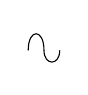
\begin{tikzpicture}[x=0.2cm,y=0.2cm]\draw (0,0) .. controls (0,1.4) and (1,1.4) .. (1,0) .. controls (1,-1) and (2,-1) .. (2,0);\end{tikzpicture}}}}

\uline{Lemme 11.14.- Soient $k$ un corps, $G$ et $H$ deux $k$-groupes affines de type fini, $u:G\handwritten{\longrightarrow}H$ un morphisme de $k$-groupes, et $u^{\unsure{o|0|\circ}}:B\handwritten{\longrightarrow}A$ l'homomorphisme de $k$-algèbres correspondant . Pour que $u$ soit fidèlement plat, il faut et il suffit que $u^o$ soit injectif.}

la condition est évidemment nécessaire (EGA IV 2.2.3 et $\unsure{0|O}_{\mathrm{IV}}$ 6.6.1). Montrons qu'elle est suffisante. Posons $K=\operatorname{Ker}u$. Alors $G/K$ est un $k$-groupe\inserted{ de type fini} (\deleted{Exp.} $\mathrm{VI}_A$ 5.2), et $u$ se factorise en $G\overset{\inserted{p}}{\handwritten{\longrightarrow}}\deleted{\unsure{p}}G/K\overset{v}{\handwritten{\longrightarrow}}H$, où $p$ est fidèlement plat (\deleted{Exp.} $\mathrm{VI}_A$ 3.2) et où $v$ est un monomorphisme de $k$-groupes de type fini, donc une immersion fermée (1.4.2). Puisque $H$ est un schéma affine, et que $v$ est une immersion fermée, $G/K$ est un schéma affine (\unsure{FGA|EGA} I 4.2.3), et, si on note $C$ l'algèbre de $G/K$, l'homomorphisme $v^o:B\handwritten{\longrightarrow}C$ est surjectif (loc. cit.) Or, puisque $u^o$ est injectif, et que $u^o=p^o\mathbin{o}v^o$, $v^o$ est aussi injectif : c'est un isomorphisme, donc $v$ est un isomorphisme, et, puisque $p$ est fidèlement plat, il en est de même de $u$.

\uline{Définitions 11.15}.- Etant donné un corps $k$, un $k$-espace vectoriel $V$, un $k$-groupe $G$ opérant sur $V$, et un vecteur $v\in V$, on dit que $v$ est \uline{semi-invariant} sous $G$ si le sous-espace vectoriel $\handwritten{k.v}$ \deleted{soit}\handwritten{est} stable sous $G$.
\margin{\figure{\handwritten{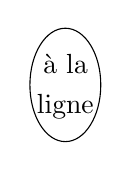
\begin{tikzpicture}[x=0.45cm,y=0.45cm]\draw (0,0) ellipse (1 and 1.6);\node at (0,0.6) {à la};\node at (0,-0.6) {\unsure{ligne}};\end{tikzpicture}}}}
\figure{\handwritten{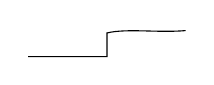
\begin{tikzpicture}[x=0.5cm,y=0.3cm]\draw (0,0) -- (2,0) -- (2,1) .. controls (2.5,1.2) and (3.3,1) .. (4,1.1);\end{tikzpicture}}}
Notons $A$ l'algèbre de $G$, et $\handwritten{\rho}:V\handwritten{\longrightarrow}A\handwritten{\otimes}_k V$ l'application linéaire qui définit l'opération de $G$ sur $V$. Dire que $v$ est semi-invariant sous $G$ revient à dire \deleted{que, pour} qu'il existe $\handwritten{\lambda}\in A$ tel que, pour tout $w\in kv$, $\handwritten{\rho}(w)=\handwritten{\lambda\otimes}w$. Lorsque $v\handwritten{\neq}0$, l'élément $\handwritten{\lambda\in}A$ est bien déterminé par cette relation, on l'appellera \deleted{\uline{invariant}}\inserted{\handwritten{\uline{poids}}} de l'élément semi-invariant $\handwritten{v}$.

\deleted{D'autre part, $v$ s'interprète comme un élément du bidual de $V$, donc comme une section de $\handwritten{\unsure{\mathbb{V}|V}}(V)$; notons $\handwritten{\varphi}:G\handwritten{\times\mathbb{V}}(V)\handwritten{\longrightarrow\mathbb{V}}(V)$ le morphisme définissant l'opération de $G$ sur $\handwritten{\mathbb{V}}$.} Dire que $v$ est semi-invariant \deleted{revient à dire qu'il existe $\unsure{g\in k|\lambda\in k}$} d'invariant $\handwritten{\lambda}$ revient à dire que $\handwritten{\varphi}(g,v)=\handwritten{\unsure{\widetilde{\lambda}|\chi|\lambda}}(g)v$ pour tout $g\in G(k)$, où $\deleted{\handwritten{\unsure{\chi:G\longrightarrow\underline{G}_{m,k}}}}\inserted{\handwritten{\widetilde{\lambda}:G\longrightarrow\underline{G}_{m,k}}}$ est le morphisme défini par $\handwritten{\lambda}$. On voit donc que $\handwritten{\lambda}$ \deleted{correspond à}\inserted{\handwritten{est}} un caractère \deleted{\handwritten{\unsure{$\chi$}}} de $G$, appelé \uline{caractère associé} à l'élément semi-invariant $v$. \deleted{Enfin nous appellerons poids de l'élément semi-invariant $v$ le poids du caractère $\handwritten{\chi}$ associé à $v$.}
\margin{\handwritten{!}}
\scanpage{54}
\mspage{\handwritten{22}}
% archive sheet number: 53

\uline{Théorème 11.16.}- (Chevalley). Soient $k$ un corps, $G$ un $k$-groupe algébrique affine, $H$ un sous-préschéma en groupes fermé de $G$. Alors il existe un nombre fini d'éléments $a_i$ linéairement indépendants de l'algèbre $A$ de $G$, tels que $H$ soit le plus grand sous-préschéma en groupes fermé de $G$ sous lequel les $a_i$ soient semi-invariants; on peut de plus supposer que tous les $a_i$ ont même \deleted{caractère associé (donc même} poids\deleted{)} sous $H$.

Rappelons que, puisque $G$ est affine, il en est de même de $H$ (\deleted{Exp.} I 4.2.3). Soit $A$ (resp. $B$) l'algèbre de $G$ (resp. $H$); d'après \deleted{\handwritten{\unsure{§}}}EGA I 4.2.3, il existe un idéal $I$ de $A$ tel que $B$ \unsure{qoit|soit} isomorphe à $A/I$. Puisque $G$ opère sur lui-même par translations à gauche, il opère aussi sur $A$, cette opération se traduisant par l'application diagonale $\handwritten{\Delta}:A\handwritten{\longrightarrow}A\handwritten{\otimes}_k A$ (\deleted{Exp.} I 4.2 et 4.7.2). Puisque $G$ est de type fini sur $k$, $A$ est de type fini sur $k$, donc $I$ \deleted{\unsure{ad}} admet un système fini de générateurs $(g_1,\ldots,g_r)$. Il résulte de (11.9) qu'il existe un sous-espace vectoriel $V$ de dimension finie de $A$ \deleted{\unsure{sat}} stable sous $G$, et contenant chacun des $g_i$.

\margin{\figure{\handwritten{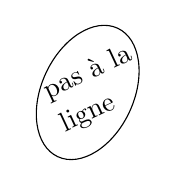
\begin{tikzpicture}[x=0.45cm,y=0.45cm]\draw[rotate=-25] (0,0) ellipse (1.3 and 2);\node[rotate=25] at (0,0.55) {pas à la};\node[rotate=25] at (0,-0.6) {ligne};\end{tikzpicture}}}}
\margin{\figure{\handwritten{\begin{tikzpicture}[x=0.3cm,y=0.3cm]\draw (1,0.8) .. controls (-0.5,1.5) and (-1,0) .. (1,0.2);\end{tikzpicture}}}}
Posons alors $W=V\handwritten{\cap}I$, c'est un espace vectoriel sur $k$ de dimension finie, dont nous noterons $d$ la dimension. Puisque $V$ contient tous les $g_i$, $W$ engendre \deleted{l'algèbre}\inserted{\handwritten{l'ideal}} $I$.

\margin{\figure{\handwritten{\begin{tikzpicture}[x=0.3cm,y=0.3cm]\draw (1,0.8) .. controls (-0.5,1.5) and (-1,0) .. (1,0.2);\end{tikzpicture}}}}
Notons $p:A\handwritten{\longrightarrow}A/I=B$ l'application canonique, et $q=p\handwritten{\otimes}\operatorname{id}_A:A\handwritten{\otimes}_k A\handwritten{\longrightarrow}(A/I)\handwritten{\otimes}_k A$ Alors l'action de $H$ sur $A$ est déterminée par $q\mathbin{o}\handwritten{\Delta}:A\handwritten{\longrightarrow}B\handwritten{\otimes}_k A$. Puisque $H$ est un sous-préschéma en groupes de $G$, l'application diagonale $A/I\handwritten{\longrightarrow}(A/I)\handwritten{\otimes}_k(A/I)=((A/I)\handwritten{\otimes}_k A)/((A/I)\handwritten{\otimes}_k I)$ se déduit de $q\mathbin{o}\handwritten{\Delta}$ par passage au quotient, ce qui montre que $(q\mathbin{o}\handwritten{\Delta})(I)\subset(A/I)\handwritten{\otimes}_k I$, autrement dit, $I$ est stable sous $H$. Puisque $V$ est stable sous $G$, donc sous $H$, on voit que $W$ est stable sous $H$.

Posons $E=\handwritten{\wedge}^d V$, soit $(w_1,\ldots,w_d)$ une base de $W$ sur $k$, et soit $(e_{\unsure{o|0}},\mathinner{..},e_n)$ une base de $E$ sur $k$ contenant $e_o=w_1\handwritten{\wedge}\cdots\handwritten{\wedge}w_d$. L'opération de $G$ sur $\handwritten{V}$ détermine canoniquement une opération de $G$ sur $\handwritten{\wedge}^d V$, qui définit une application linéaire $\handwritten{\rho}:E\handwritten{\longrightarrow}A\handwritten{\otimes}_k E$. Posons $\handwritten{\rho}(e_i)=\handwritten{\sum}a_j^i\handwritten{\otimes}e_j$, et $a_i=a_i^o$. Puisque $W$ est stable sous $H$, si on pose $\handwritten{\sigma}=(p\handwritten{\otimes}\operatorname{id}_E)\mathbin{o}\handwritten{\rho}:E\handwritten{\longrightarrow}(A/I)\handwritten{\otimes}_k E$, il est clair que $\handwritten{\sigma}(e_o)$ est proportionnel à $e_o$, autrement dit, pour $1\leqq i\leqq n$, on a $a_i\in I$. L'axiome (CM1) de (\deleted{Exp.} I \unsure{4.72|4.7.2}) appliqué à
\scanpage{55}
\mspage{\handwritten{23}}
% archive sheet number: 54

$\handwritten{\rho}(e_{\unsure{o|0}})=\handwritten{\sum}a_i\handwritten{\otimes}e_i$ montre que $\handwritten{\sum\Delta}(a_i)\handwritten{\otimes}e_i=\handwritten{\sum}a_i\handwritten{\otimes\rho}(e_i)=\handwritten{\sum}a_i\handwritten{\otimes}a_j^i\handwritten{\otimes}e_j$, d'où on déduit que $\handwritten{\Delta}(a_i)=a_o\handwritten{\otimes}a_i+\handwritten{\sum_{j\geq1}}a_j\handwritten{\otimes}a_i^j$; donc, puisque pour $j\geq1$, $a_j\in I$, on voit que $q\mathbin{o}\handwritten{\Delta}(a_i)=p(a_o)\handwritten{\otimes}a_i$, si bien que pour $1\leqq i\leqq n$, $a_i$ est semi-invariant sous $H$ \deleted{\unsure{d'invara}} \deleted{d'invariant}\inserted{\handwritten{de poids}} $p(a_o)$, indépendant de $i$; \deleted{donc tous les $a_i$ sont semi-invariants sous $H$ de même caractère associé, donc de même poids. Enfin}\inserted{\handwritten{Extrayons}} du système $(a_1,\ldots,a_n)$, \deleted{on peut extraire} un système maximal de vecte\deleted{\unsure{ur}}\handwritten{\unsure{ur}}s linéairement indépendants, dont on peut supposer qu'il se note $(a_{\handwritten{1}},\mathinner{..},a_m)$. \inserted{\handwritten{Alors les $a_i$, $i=1,\unsure{\mathinner{-\,-}|\ldots},m$ sont \unsure{lineairement|linéairement} \unsure{indepdants|independants|indépendants}, semi-invariants sous $H$, et de même poids.}}

Réciproquement, soit $H'$ un sous-préschéma en groupes fermé de $G$ sous lequel chacun des $a_i$ $(1\leqq i\leqq m)$ est semi-invariant. \inserted{\handwritten{Montrons que $H'=H$}} Il existe de même un idéal $I'$ de $A$ tel que l'algèbre $B'$ de $H'$ soit isomorphe à $A/I'$; notons $p':A\handwritten{\longrightarrow}A/I'$ l'application canonique, et $q'=p'\handwritten{\otimes}\operatorname{id}_A$. Par hypothèse, pour $1\leqq i\leqq m$, il existe $\handwritten{\lambda}_i\in B'$ tel que $q'\mathbin{o}\handwritten{\Delta}(a_i)=\handwritten{\sum}p'(a_j)\handwritten{\otimes}a_i^j=\handwritten{\lambda}_i\handwritten{\otimes}a_i$. Or l'axiome (CM2) de (\deleted{Exp}I 4.7\handwritten{\unsure{.}}2) montre que $e_i=\handwritten{\sum\eta}(a_j^i)e_j$, donc que $\handwritten{\eta}(a_j^i)=\handwritten{\delta}_{ij}$ (symbole de Kronecker); l'égalité $\handwritten{\sum}p'(a_j)\handwritten{\otimes\eta}(a_j^i)=\handwritten{\lambda}_i\handwritten{\otimes\eta}(a_i)$ s'écrit donc $p'(a_i)=0$ pour $1\leqq i\leqq m$, car $\handwritten{\eta}(a_i)\handwritten{=\eta}(a_i^o)=0$ pour $1\leqq i\leqq m$; par conséquent, on a $a_i\in I'$ pour $1\leqq i\leqq m$, si bien que $a_i\in I'$ pour $1\leqq i\leqq n$. Donc, si on pose $\handwritten{\sigma}'=(p'\handwritten{\otimes}\operatorname{id}_E)\mathbin{o}\handwritten{\Delta}$, $\handwritten{\sigma}'(e_o)=\handwritten{\sum}p'(a_i)\handwritten{\otimes}e_i$ est proportionnel à $e_o$, de sorte que $q'\mathbin{o}\handwritten{\Delta}(W)\subset A/I'\handwritten{\otimes}_k W$, autrement dit que $W$ est stable sous $H'$. Puisque $W$ engendre\inserted{\handwritten{ l'ideal}} $I$, $I$ est stable sous $H'$, donc $q'\mathbin{o}\handwritten{\Delta}(I)\subset(A/I')\handwritten{\otimes}_k I$, et $q'\mathbin{o}\handwritten{\Delta}$ définit par passage au quotient une application linéaire $A/I\handwritten{\longrightarrow}(A/I')\handwritten{\otimes}_k(A/I)\handwritten{=((A/I')\otimes_k A)/((A/I')\otimes_k I)}$ donc \deleted{\illegible{14}}\inserted{la restriction à $H'\handwritten{\times_k}H$ du morphisme de multiplication de $G$ se factorise à travers $H$}, ce qui implique que $H'$ est \deleted{inclus dans $H$, c.q.f.d.} un sous-préschéma en groupes de $H$, c.q.f.d.

\margin{\handwritten{\unsure{le th. est} \unsure{une} \illegible{3} \unsure{11} (\unsure{voir la fin}) \unsure{j'ai|j'écris} \illegible{3} \unsure{en} \illegible{2} \unsure{élémentaire|démonstration}}}
\uline{Théorème} \uuline{11.17} (Chevalley).- Soient $k$ un corps, $G$ un $k$-groupe affine (non nécessairement algébrique), et $H$ un sous-préschéma en groupes fermé de $G$ \uline{invariant} dans $G$; alors le faisceau quotient (pour la topologie fpqc) $G/H$ est représentable par un $k$-groupe \uline{affine}.

\margin{\figure{\handwritten{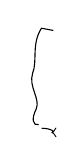
\begin{tikzpicture}[x=0.35cm,y=0.35cm]
\draw[thin] (0.45,3.5) -- (0.02,3.58) .. controls (-0.35,3.0) and (-0.12,2.4) .. (-0.30,1.95) .. controls (-0.46,1.45) and (-0.01,1.03) .. (-0.17,0.65) .. controls (-0.35,0.30) and (-0.30,0.03) .. (-0.08,0.08);
\draw[thin,->] (0.03,-0.05) .. controls (0.40,-0.05) and (0.52,-0.20) .. (0.38,-0.20);
\end{tikzpicture}}}}
\uline{Premier cas} : \handwritten{S}upposons d'abord $G$ algébrique. D'après (\deleted{\unsure{Exp.}} $\mathrm{VI}_A$ 3.2), le conoyau $K$ de l'injection $H\handwritten{\longrightarrow}G$ existe, \deleted{et} le morphisme canonique $p:G\handwritten{\longrightarrow}K$ est \deleted{fidèlement plat , et quasi-compact, puisque $G$ est de type fini sur $k$, et que $K$, qui est muni d'une structure de $k$-groupe (Exp. $\mathrm{VI}_A$ 5.2) est séparé sur $k$ (Exp. $\mathrm{VI}_A$ 0.2). Donc $p$ est} couvrant pour la topologie fpqc, \deleted{si bien (\deleted{\unsure{Exp.}} IV 4.4.3) que}\inserted{\handwritten{et}} $K$ représente le faisceau quotient $G/H$ pour la topologie fpqc;
\scanpage{56}
% archive sheet number: 55

\handwritten{Supposons d'abord $k$ algébriquement clos, $G$ réduit et connexe et $H$ réduit. D'après (\uline{BIBLE} \deleted{\unsure{VII|VIII}}\inserted{\deleted{Exp} 4, cor du th.\uline{1}}), il existe une représentation linéaire de dimension finie $\rho:G\longrightarrow\mathrm{GL}(V)$ telle que $(\operatorname{Ker}\rho)_{\mathrm{red}}=H$. Par 11.11, $G/\operatorname{Ker}\rho$ est affine. donc $(G/H)/(\operatorname{Ker}\rho/H)$ est affine, donc aussi $G/H$, le groupe $\operatorname{Ker}\rho/H$ étant fini.}

\handwritten{Si $k$ est algébriquement clos, et $G$ et $H$ réduits, alors $(G/H)/(G^{\unsure{\circ|0|o}}/H\cap G^\circ)$ est fini,\inserted{ comme quotient de $G/G^\circ$, et} $G^\circ/H\cap G^\circ$ est affine, donc $G/H$ est affine.}
\margin{\figure{\handwritten{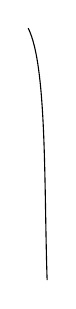
\begin{tikzpicture}[x=0.2cm,y=0.4cm]\draw (0,8) .. controls (1.2,6.8) and (1,3) .. (1.2,0);\end{tikzpicture}}}}

\figure{\handwritten{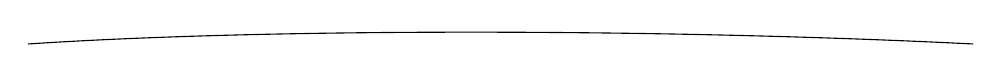
\begin{tikzpicture}\draw (0,0) .. controls (3,0.2) and (8,0.2) .. (12,0);\end{tikzpicture}}}
\deleted{\handwritten{\uline{N.B.}1) le th \unsure{entraîne|entraine} que si $G$ est affine algébrique et $H$ invariant, il existe \unsure{un|une} rep linéaire de dim finie $\rho:G\longrightarrow\mathrm{GL}(V)$ telle que $H=\operatorname{Ker}\rho$}}

\deleted{\handwritten{2) La réf à BIBLE est un corollaire de 11.16, la démonstration est facile mais un peu longue.}}

\deleted{\handwritten{3) \unsure{Dan|Dans} la réf à BIBLE Supposer $G$ connexe, car la dém. de BIBLE est \unsure{erronée} dans le cas général}}
\figure{\handwritten{\begin{tikzpicture}\draw (0,0) .. controls (4,0.4) and (8,0.5) .. (12,0.6);\end{tikzpicture}}}
\scanpage{57}
\mspage{\handwritten{24}}
% archive sheet number: 56

il s'agit donc de montrer que $K$ est affine.

\deleted{Le théorème est connu dans le cas où $k$ est algébriquement clos et où $G$ et $H$ sont réduits (Chevalley}\deleted{\unsure{)}}\inserted{\deleted{\handwritten{Supposons d'abord}}}.
\margin{\figure{\handwritten{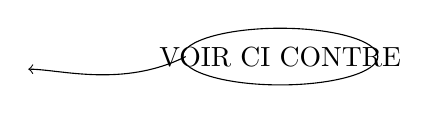
\begin{tikzpicture}[x=0.4cm,y=0.4cm]\draw (0,0) ellipse (3.1 and 0.9);\node at (0,0) {VOIR CI CONTRE};\draw[->] (-3,0) .. controls (-5,-1) and (-7,-0.4) .. (-8,-0.4);\end{tikzpicture}}}}

Dans le cas où $k$ est algébriquement clos, et $G$ et $H$ quelconques,\deleted{(\unsure{$(G/H)_{\mathrm{red}}$} est isomorphe à \unsure{$G_{\mathrm{red}}/H_{\mathrm{red}}$} réduit (\unsure{9.2 vi|9.2 iv})}, $(G\handwritten{\times}_k H)_{\mathrm{red}}$ est isomorphe à $(G_{\mathrm{red}})\handwritten{\times}_k(H_{\mathrm{red}})$, donc $(G_{\mathrm{red}})/(H_{\mathrm{red}})$ est isomorphe à $(G/H)_{\mathrm{red}}$. Puisque $(G_{\mathrm{red}})/H_{\mathrm{red}}$ est affine, il en est de même de $G/H$ (EGA I 5.1.10), car, puisque $G/H$ est de type fini sur $k$, son nilradical est nilpotent.

Dans le cas où $k$ est quelconque, $G\handwritten{\otimes}_k\handwritten{\bar{k}}/H\handwritten{\otimes}_k\handwritten{\bar{k}}$ est isomorphe à $(G/H)\handwritten{\otimes}_k\handwritten{\bar{k}}$ (9.2 v)), donc puisque le premier est affine, il en est de même du second, donc $G/H$ est affine\handwritten{(ref.)\unsure{,|'}}
\margin{\handwritten{(\qquad)}}

\uline{Deuxième cas} : \handwritten{C}as général . D'après (11.13), l'algèbre $A$ de $G$ est limite inductive d'une famille filtrante croissante $(A_i)_{i\in I}$ de sous-algèbres de type fini de $A$ stables par l'application diagonale et l'involution. D'après (\deleted{Exp.}\inserted{EGA} I 4.2.3), $H$ est affine, et si on note $B$ l'algèbre de $H$, l'homomorphisme $A\handwritten{\longrightarrow}B$ déduit de l'injection $H\handwritten{\longrightarrow}G$ est surjectif. Posons $I=\operatorname{Ker}(A\handwritten{\to}B)$, $I_i=I\handwritten{\cap}A_i$ et $B_i=A_i/I_i$; puisque la structure d'hyperalgèbre associative augmentée involutive de $A$ passe au quotient à travers $I$, on vérifie aisément que celle de $A_i$ passe au quotient à travers $I_i$, si bien que $B_i$ est l'algèbre d'un $k$-groupe affine de type fini $H_i$; il est clair que $B=\lim B_i$. D'après (EGA I 4.2.3), $H_i$ est isomorphe à un sous-préschéma en g\inserted{\handwritten{r}}oupes fermé de $G_i$. D'après (6.7) le fait que $H$ soit invariant dans $G$ s'exprime en disant qu'un certain morphisme $H\handwritten{\times}_k G\handwritten{\longrightarrow}G$ se factorise à travers l'injection $H\handwritten{\longrightarrow}G$, autrement dit que l'homomorphisme correspondant $A\handwritten{\longrightarrow}B\handwritten{\otimes}_k A$ se factorise à travers l'homorphisme canonique $A\handwritten{\longrightarrow}B$; on vérifie aisément que l'homomorphisme $A_i\handwritten{\longrightarrow}B_i\handwritten{\otimes}_k A_i$ défini de manière analogue se factorise à travers $A_i\handwritten{\longrightarrow}B_i$, donc que $H_i$ est invariant dans $G_i$. D'après ce qui a été vu précédemment, $G_i$ étant de type fini sur\inserted{\handwritten{\ }}$k$, $G_i/H_i$ est représentable par un $k$-groupe affine $K_i$, dont nous noterons $C_i$ l'algèbre. Posons alo\deleted{r}\handwritten{\unsure{r|4}}s $C=\underset{\handwritten{\longrightarrow}}{\lim}C_i$, et soit $K=\underset{\handwritten{\longleftarrow}}{\lim}K_i$ le $k$-préschéma affine d'algèbre $K$ (EGA IV 8.2.3).

Montrons que $K$ représente $G/H$; pour cela, il suffit de vérifier que \deleted{le diagramme}
\margin{\handwritten{\unsure{est ce défini ?}}}
\diagram{\begin{tikzcd}[ampersand replacement=\&,execute at end picture={\draw[thin] (current bounding box.center) ellipse [x radius=4.2cm,y radius=0.55cm];}]
H\handwritten{\times}_k G \arrow[r,"\handwritten{\sim}"] \& G\deleted{\unsure{\longrightarrow K}}\handwritten{\times_K G}\quad\text{\deleted{est cartésien}}
\end{tikzcd}}
\handwritten{,} et que le morphisme $G\handwritten{\longrightarrow}K$ est couvrant pour la topologie fpqc. (\deleted{\unsure{Exp.}} IV 4.4.3). Or, \deleted{chacun des diagrammes}\inserted{\handwritten{pour chaque $i$, on \unsure{a}}}
\diagram{\begin{tikzcd}[ampersand replacement=\&]
H_i\handwritten{\times}_k G_i \arrow[r,"\handwritten{\sim}"] \& G_i\deleted{\unsure{\longrightarrow K_i}}\handwritten{\times_{K_i}G_i}
\end{tikzcd}}
\handwritten{,}\deleted{étant cartésien,}\inserted{\handwritten{donc}} il en est de même d\deleted{\unsure{u|e}}\handwritten{\unsure{u}} \deleted{diagramme}\inserted{\handwritten{morphisme}} obtenu en passant à la limite projective; enfin chacun des morphismes
\scanpage{58}
\mspage{\handwritten{25}}
% archive sheet number: 57

$G_i\handwritten{\longrightarrow}K_i$ est fidèlement plat (9.2 (xi)), autrement dit $C_i$ est fidèlement plat sur $A_i$; puisque $A=\underset{\handwritten{\longrightarrow}}{\lim}A_i$ et $C=\underset{\handwritten{\longrightarrow}}{\lim}C_i$, on en déduit que $C$ est fidèlement plat sur $A$\handwritten{,}\deleted{(cf. \unsure{Bourbaki} Alg. Comm. \illegible{3})} si bien que $G\handwritten{\longrightarrow}K$ est un morphisme fidèlement plat. Puisque ce morphisme est affine, il est quasi-compact, donc couvrant pour la topologie fpqc,c.q.f.d.

\deleted{\uline{Corollaire} 11.18. Soient $k$ un corps, $G=D(M)$ un groupe diagonalisable sur $k$ (I 4.4), \deleted{$H$ un sous-groupe de} avec $M$ un $\text{\uline{Z}}$-module de type fini, $H$ un sous-groupe algébrique de $G$. Alors $H$ est également diagonalisable.}
